%% ---------------------------------------------------------------------------------------------------------------------

\chapter{\textit{go-safer}: Detecting \textit{Unsafe} Misuses}\label{ch:go-safer}

Another major contribution of this thesis is the development of \toolSafer{}, a \toolVet{}-style, open-source linter
tool with a focus on the \unsafe{} \acrshort{API} in Go.
It can identify some of the insecure code patterns described in Chapter~\ref{ch:unsafe-security-problems}.
Figure~\ref{fig:outline5} shows the organization of this chapter.
It describes the design and implementation of \toolSafer{} based on \unsafe{}-related vulnerabilities and usage data.
Further, an evaluation of its effectiveness using the labeled data set of \unsafe{} usages introduced in the
previous chapter, a manual analysis of open-source Go packages, and a comparison with existing tools is presented.

\begin{figure}[htp!]
    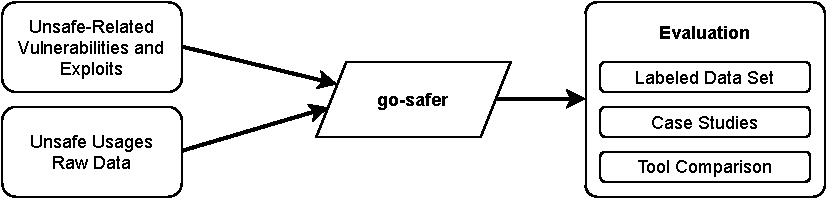
\includegraphics[width=\textwidth]{assets/figures/chapter5/outline5.pdf}
    \caption{Role of Chapter 5 in the thesis outline}
    \label{fig:outline5}
\end{figure}



%% ---------------------------------------------------------------------------------------------------------------------

\section{Design}\label{sec:go-safer:design}

The \toolSafer{} static analysis tool is designed as a linter to identify \checkNum{two} misuse patterns of the
\unsafe{} \acrshort{API} that were previously undetected with existing linters such as \toolVet{} and \toolGosec{}.
These patterns are automatically detectable using static analysis.
For some vulnerabilities discussed in Chapter~\ref{ch:unsafe-security-problems}, this is not possible or too hard for
the scope of this thesis.
The selection of the code patterns that are detected is based on the \unsafe{} usage examples identified using
\toolGeiger{} in popular open-source Go projects as described in
Section~\ref{subsec:go-geiger:qualitative-evaluation:labeled-dataset}, as well as the manual analysis of possible
vulnerabilities related to the use of the \unsafe{} \acrshort{API} presented in
Chapter~\ref{ch:unsafe-security-problems}.
The first is the incorrect conversion pattern between slices and strings by creating their header structures as
composite literals as described in Section~\ref{subsec:unsafe-security-problems:slice-casts:gc-race}.
Listing~\ref{lst:go-safer-sliceheader-pass} shows a code example that uses this pattern.
The insecure creation of a \textit{reflect.SliceHeader} instance is done in Lines~3--7.

\begin{lstlisting}[language=Golang, float, label=lst:go-safer-sliceheader-pass, caption=First vulnerable code pattern detected by \toolSafer{}]
func unsafeFunction(s string) []byte {
    sH := (*reflect.StringHeader)(unsafe.Pointer(&s))
    bH := &reflect.SliceHeader{
        Data: sH.Data,
        Len:  sH.Len,
        Cap:  sH.Len,
    }
    return *(*[]byte)(unsafe.Pointer(bH))
}
\end{lstlisting}


In addition to composite literals of type \textit{reflect.SliceHeader} and \textit{reflect.StringHeader}, \toolSafer{}
analyzes accesses to fields of existing instances of these types, unless they are derived by cast from a real slice or
string.
If they are, then their \textit{Data} field is treated as a reference by the Go runtime, as described in
Section~\ref{sec:background:slices}.
Furthermore, if the slice or string header types are renamed to a different type name in the source code, field accesses
and composite literals of the new type name are recognized just like the original types.

The second misuse that \toolSafer{} detects is a direct conversion between struct types containing incompatible types
with architecture-dependent sizes or alignments as described in
Section~\ref{sec:unsafe-security-problems:architecture-dependent-types}.
Listing~\ref{lst:go-safer-structcast-pass} shows an example of such code.
Here, Line~8 contains an incorrect cast between the incompatible structures \textit{A} (Lines~1--3) and \textit{B}
(Lines~4--6).

\begin{lstlisting}[language=Golang, label=lst:go-safer-structcast-pass, caption=Second vulnerable code pattern detected by \toolSafer{}]
type A struct {
    x int
}
type B struct {
    y int64
}
func unsafeFunction(a A) B {
    return *(*B)(unsafe.Pointer(&a))
}
\end{lstlisting}


The source code and documentation of \toolSafer{} is available on
\github{}\footnote{\url{https://github.com/jlauinger/go-safer}}.
Figure~\ref{fig:go-safer-screenshot} shows a screenshot of \toolSafer{}.
The output contains a few warnings about insecure slice conversions, which are detected in the \textit{nil\_cast}
package that is part of the \toolSafer{} test suite.
For each warning, one line is generated in the output including the source file, line number, and column of the insecure
code.

\begin{figure}[htp!]
    %\vspace{2mm}
    \centering
    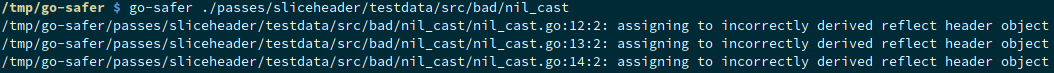
\includegraphics[width=\textwidth]{assets/images/chapter5/go-safer-screenshot.png}
    \caption{Usage example screenshot of \toolSafer{}}
    \label{fig:go-safer-screenshot}
    %\vspace{-14pt}
\end{figure}



%% ---------------------------------------------------------------------------------------------------------------------

\section{Implementation}\label{sec:go-safer:implementation}

The \toolSafer{} tool is built using the Go analysis infrastructure that is available as part of \toolVet{}.
This allows to compose analysis steps as modular and reusable parts, which are called \textit{passes}.
Each analysis pass is run as a unit on the source code packages under analysis.
It can depend on the results of other analysis passes, which are run before and hand the results over to it.
The passes and their relations must form a directed acyclic graph, and the analysis infrastructure code determines the
optimal execution order and concurrency.
There are two novel analysis passes in \toolSafer{}, the \textit{sliceheader} and the \textit{structcast} pass.
Figure~\ref{fig:go-safer-architecture} shows an overview of this architecture.

\begin{figure}[!t]
    \vspace{2mm}
    \centering
    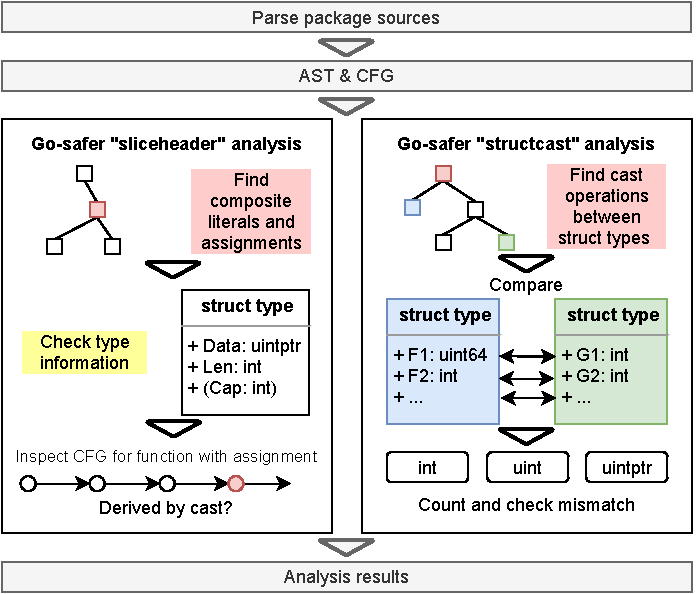
\includegraphics[width=0.48\textwidth]{gfx/figures/go-safer-architecture.pdf}
    %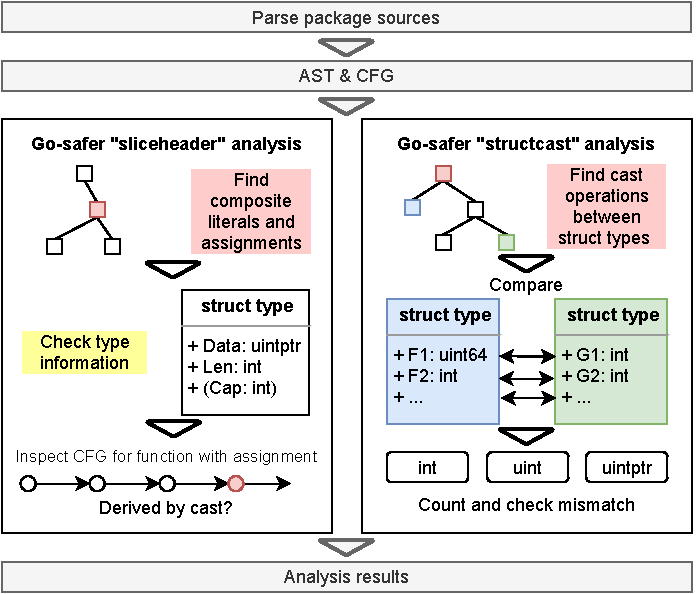
\includegraphics[width=0.45\textwidth]{gfx/figures/go-safer-architecture.pdf}
    \caption{Architecture of \toolSA{} static code analysis tool}
    \label{fig:safer-architecture}
    %\vspace{-14pt}
\end{figure}


Parts that are shown in gray in Figure~\ref{fig:go-safer-architecture} are reusing existing code.
Parsing the source code of the packages under analysis is done in the same way that \toolVet{} does, in fact that code
is imported as a dependency for \toolSafer{}.
Then, the abstract syntax tree (\acrshort{AST}) and control flow graph (\acrshort{CFG}) of the sources are built using
existing analyses, which the novel \toolSafer{} passes depend upon.
After all analyses are finished, the results are presented to the user.
This composition using many existing parts allows to keep the required new code to a minimum, reuses well-tested pieces
of code, and allows integrating the new \toolSafer{} features into a familiar workflow.

The \textit{sliceheader} analysis pass finds the code pattern shown in Listing~\ref{lst:go-safer-sliceheader-pass}.
First, it receives the \acrshort{AST} and filters it for composite literals (\textit{CompositeLit} nodes) and
assignment statements (\textit{AssignStmt} nodes).
Recursively going down the \acrshort{AST} even after a composite literal has been found ensures that \toolSafer{} also
detects literals that are part of a bigger structure type that contains a slice header as one of its fields.
Then, the type of either the composite literal or the assignment receiver is checked.
For assignments, this is done by looking up the left hand side identifier in a type table provided by the parser.
Since Go supports multiple assignments in one statement, there can be multiple variables on the left hand side.
In this case, \toolSafer{} checks all of them to see if any meet the conditions to trigger a warning.
To check whether the type matches either \textit{reflect.StringHeader} or \textit{reflect.SliceHeader}, it is checked
for assignability to the underlying structure of the header types.
This structure, as illustrated in Figure~\ref{fig:go-safer-architecture}, is one \textit{uintptr} field, and one or two
\textit{int} fields.
Comparing to the structure instead of the name of the type makes it possible to detect type aliases of the header types
which might exist.
An example of this is shown in Listing~\ref{lst:go-safer-sliceheader-alternative-code}.
It contains a type definition for \textit{CustomHeader} (Line~1), which is then used to create a composite literal
(Lines~4--8).

\begin{lstlisting}[language=Golang, label=lst:go-safer-sliceheader-alternative-code, caption=\textit{SliceHeader} alias type detected by \toolSafer{}]
type MyHeader reflect.SliceHeader

func unsafeFunction(address uintptr) []byte {
    header := &MyHeader{
        Data: address,
        Len:  42,
        Cap:  42,
    }
    return *(*[]byte)(unsafe.Pointer(header))
}
\end{lstlisting}


A composite literal of a header type is enough to issue a warning, but for assignments, \toolSafer{} needs to check
whether the receiver variable is a slice or string header that was created by conversion from a real slice or string.
To do this, the \acrshort{AST} assignment node is identified within the \acrshort{CFG}.
Then, going backwards in the \acrshort{CFG}, the last node that assigns the value of the receiver variable is found.
This node defines the effective value of the slice or string header structure at the time of the assignment under
investigation.
Finally, \toolSafer{} checks whether the right hand side value of the statement defining that value is a conversion
from an actual slice or string value.
It has to be a cast through an \textit{unsafe.Pointer} value for this to be possible.
If that is the case, the assignment is legitimate and \toolSafer{} does not generate a warning.
However, if the variable is not derived by a conversion from a slice or string, or no \acrshort{CFG} node defining the
variable can be found, a warning is issued.
This is possible, for example, if the slice or string header is passed as a function parameter, because its value can
not be statically inferred with the Go analysis framework in that case.

The \textit{structcast} pass is responsible for detecting the code pattern shown in
Listing~\ref{lst:go-safer-structcast-pass}.
It also uses the \acrshort{AST} to find cast operations.
These are represented in the \acrshort{AST} in the same way as function calls are, so the tree is filtered for
\textit{CallExpr} nodes.
If there is a cast from some structure type to \textit{unsafe.Pointer} and further to another structure type, these
source and target types are analyzed.
These types can again be fetched from a type lookup table provided by the parser.
For both of them, \toolSafer{} counts the number of fields that have the types \textit{int}, \textit{uint}, or
\textit{uintptr}.
These \checkNum{three} basic types are the ones available in Go that have different sizes, alignments, and byte orders
on varying architectures.
For example, \textit{int} is \checkNum{eight} bytes on the \textit{amd64} architecture, but only \checkNum{four} bytes
on \textit{i386}.
If the counts mismatch, the direct cast using the \unsafe{} \acrshort{API} will likely break on some architectures,
and \toolSafer{} generates a warning.


%% ---------------------------------------------------------------------------------------------------------------------

\section{Evaluation}\label{sec:go-safer:evaluation}

In order to make a valuable contribution to the security of Go programs, and also be an effective tool for developers,
it is important that \toolSafer{} can find actual bugs in real-world Go projects, and at the same time have a low rate
of false positives and false negatives.
False negatives would mean that the tool misses incorrect and therefore potentially vulnerable usages of the \unsafe{}
\acrshort{API}.
On the other hand, a high rate of false positives would mean that it generates many warnings that are not related to
any programming errors~\cite{banerjee2009}.
This would require developers to manually review the findings and dismiss many of them, which decreases the value of
\toolSafer{} significantly.
First, developers could lose trust in the tool and refuse using it with their regular development workflows.
Second, false positives make it hard to integrate \toolSafer{} with automated continuous integration processes, because
the build would fail without there being a real problem.

To demonstrate that \toolSafer{} is capable of finding actual bugs while having an acceptable rate of both false
positives and negatives, its performance is evaluated in two different ways.
One of them uses the novel data set of labeled \unsafe{} usages, which was presented in
Section~\ref{subsec:go-geiger:qualitative-evaluation:labeled-dataset}.
The second one is done by manually analyzing \checkNum{six} selected open-source Go packages from different projects and
comparing the results to the output of \toolSafer{}.
Finally, the performance is compared to the existing static analysis tools \toolVet{} and \toolGosec{}.

In addition to this academic evaluation, \toolSafer{} was also used to discover \numberBugsFixed{} bugs that existed in
the open-source projects used for the study on real-world usage of \unsafe{} presented in Chapter~\ref{ch:go-geiger}, or
their dependencies.
By the time this thesis was submitted, the authors of the affected projects have acknowledged \numberBugsMerged{}
(\fractionBugsMerged{}) of those bugs, and accepted the fixes that were submitted to them.


%% ---------------------------------------------------------------------------------------------------------------------

\subsection{Labeled Usages from the Data Set}\label{subsec:go-safer:evaluation:labeled-usages}

To evaluate the performance of \toolSafer{} using the novel data set of labeled \unsafe{} usages, first all instances
from the \textit{cast-header} class are taken from the set.
These are possible misuses involving incorrect constructions of slice and string headers.
There are \checkNum{44} such code samples, which are manually classified as positive and negative examples.
Positive means that the code is a misuse of the \unsafe{} \acrshort{API}, and \toolSafer{} should generate a warning for
it, while negative means that the code is a correct and safe usage.
There are \checkNum{30} positive and \checkNum{14} negative samples.

Then, \toolSafer{} is run on all packages that contain the respective \checkNum{44} \unsafe{} usage samples, and all
warnings issued are saved into a \acrshort{CSV} file.
This makes it easy to match the warnings with the labeled samples by their file name and line number.
Samples that are classified as positive are counted as true positives (TP) if \toolSafer{} generates a warning for it,
and false negative (FN) otherwise.
Similarly, negative samples count as false positives (FP) if there is a warning, and true negatives (TN) otherwise.
Table~\ref{tbl:go-safer-evaluation-dataset} shows the results of this evaluation in its first row.
The other rows contain results from other linters and are discussed in
Section~\ref{subsec:go-safer:evaluation:linters-comparison}.
Furthermore, the table contains the resulting precision, recall, accuracy, and F1-score as calculated from the classes
counts.

\begin{table}[htp!]
    \centering
    \caption{Evaluation results for \toolSafer{} on the labeled data set of \unsafe{} usages}
    \label{tbl:gosafer-evaluation-dataset}
    \begin{tabular}{l||r|r|r|r||l|l|l|l}
        \textbf{Tool} & \textbf{TP} & \textbf{FP} & \textbf{TN} & \textbf{FN} & \textbf{Precision} & \textbf{Recall} & \textbf{Accuracy} & \textbf{F1-Score} \\
        \hline
        go-safer &   29   &    1   &   13   &    1   &   0.967       &  0.967     &    0.955     & 0.967  \\
        go vet   &    0   &    0   &   14   &   30   &   -           &  0         &    0.318     & 0      \\
        gosec    &   29   &   13   &    1   &    1   &   0.690       &  0.967     &    0.681     & 0.805  \\
    \end{tabular}
\end{table}

The results show both high precision and recall of \checkNum{96.7\%} for \toolSafer{}.
High precision means that there are few false positives, so the warnings generated by \toolSafer{} are almost always
correct and show evidence of an actual bug in the code.
Therefore, developers can include it into their workflows without the need of dismissing many invalid warnings.
A high recall shows that there are few false negatives, therefore a high fraction of the existing bugs is detected by
\toolSafer{}.
Thus, developers have a reliable tool at hand to be trusted in detecting bugs of the particular class of \unsafe{}
misuses that it is specialized in.
Accuracy and F1-score are high as well, which follows from both high precision and recall and emphasizes the quality
\toolSafer{} provides.

\begin{hero}[Evaluation results on labeled usages]
    Evaluated using manually labeled \unsafe{} usages, \toolSafer{} achieves both \checkNum{96.7\%} precision and
    recall.
    Therefore, its accuracy is \checkNum{95.5\%}.
\end{hero}

A manual analysis shows that the \checkNum{one} false positive is due to a slice header that is created from a real
slice, however the slice is referenced through a slightly obfuscated, reflected pointer which \toolSafer{} can not
connect to the slice.
The false negative is caused by compilation errors in the package which prevent \toolSafer{} from analyzing the package
altogether.
Since it depends on the \acrshort{AST}, its static analysis passes can not run and the execution stops with a generic
error message before the parsing step has finished.
The same is true for \toolGosec{}.
To work around this scenario, \toolSafer{} would need a secondary analysis strategy that works on the source code
instead of the \acrshort{AST}, which is not feasible with the tools presented in this thesis.


%% ---------------------------------------------------------------------------------------------------------------------

\subsection{Case Study Packages}\label{subsec:go-safer:evaluation:case-studies}

A second evaluation of \toolSafer{} is done by manually analyzing \checkNum{six} selected Go packages from open-source
projects.
These packages are chosen using the results of the study on \unsafe{} usage in open-source code presented in
Section~\ref{sec:go-geiger:quantitative-evaluation}.
Evaluating \toolSafer{}, an \unsafe{}-related linter, on packages that do not actually contain any \unsafe{} usages does
not provide valuable insights.
Table~\ref{tbl:go-safer-evaluation-packages-stats} shows the \checkNum{six} packages used for this evaluation, including
their number of Go files, lines of code (\acrshort{LOC}), and \unsafe{} usages.
They are manually selected from the packages in the dependency trees of the projects analyzed with \toolGeiger{}.
To create a variation both of the number of \unsafe{} usages and package size, they are chosen to include two packages
each with few, medium, and many \unsafe{} usages.
For every category, there is one small and one large package in terms of \acrshort{LOC} each.

\begin{table}[htp!]
    \centering
    \caption{Selected packages for the evaluation of \toolSafer{}}
    \label{tbl:go-safer-evaluation-packages-stats}
    \begin{tabular}{l|r|r|r}
        \textbf{Package}                        & \textbf{Number of Go Files} & \textbf{\acrshort{LOC}} & \textbf{Unsafe Usages} \\
        \hline
        k8s.io/kubernetes/pkg/apis/core/v1      & 6                           & 10,048                  & 677                    \\
        \rowcolor{verylightgray}
        gorgonia.org/tensor/native              & 4                           & 1,867                   & 158                    \\
        github.com/anacrolix/mmsg/socket        & 86                          & 3,782                   & 115                    \\
        \rowcolor{verylightgray}
        github.com/cilium/ebpf                  & 14                          & 2,851                   & 65                     \\
        golang.org/x/tools/internal/event/label & 1                           & 213                     & 8                      \\
        \rowcolor{verylightgray}
        github.com/mailru/easyjson/jlexer       & 4                           & 1,234                   & 5                      \\
        \hline
        \textbf{Total}                          & \textbf{115}                & \textbf{19,995}         & \textbf{1,028}         \\
    \end{tabular}
\end{table}

The \checkNum{six} packages were analyzed manually to find any insecure code that \toolSafer{} should detect.
The results of this were saved as a \acrshort{CSV} file containing a positive or negative label for every line of code
that includes a usage of the \unsafe{} \acrshort{API}.
Lines that do not use the \acrshort{API} should not be analyzed by \toolSafer{} at all, therefore they are not included
as negative in order to avoid a very large number of true negatives which would skew the accuracy and yield less
valuable evaluation results.
Should \toolSafer{} generate a warning for such a line, it will still be counted as false positive.
After the manual analysis, \toolSafer{} was run on the packages.
Similar to Section~\ref{subsec:go-safer:evaluation:labeled-usages}, the warnings and labels were matched and counted.

\begin{table}[htp!]
    \centering
    \caption[Evaluation results for \toolSafer{} on manually analyzed packages packages]
        {Evaluation results for \toolSafer{} on manually analyzed packages packages~\newline \tiny ~\newline \footnotesize
        Tools: \underline{a} \toolSafer{}, \underline{b} \toolVet{}, \underline{c} \toolGosec{} \tiny ~\newline}
    \label{tbl:go-safer-evaluation-packages}
    \begin{adjustbox}{max width=\textwidth}
        \begin{tabular}{l||rrr|rrr|rrr|rrr||lll|lll|lll|lll}
            \textbf{Package} & \multicolumn{3}{c|}{\textbf{TP}}                & \multicolumn{3}{c|}{\textbf{FP}}                   & \multicolumn{3}{c|}{\textbf{TN}}                    & \multicolumn{3}{c||}{\textbf{FN}}                  & \multicolumn{3}{c|}{\textbf{Precision}}  & \multicolumn{3}{c|}{\textbf{Recall}}    & \multicolumn{3}{c|}{\textbf{Accuracy}}           & \multicolumn{3}{c}{\textbf{F1-Score}}    \\
            {}               & \textit{a}            & \textit{b} & \textit{c} & \textit{a}             & \textit{b} & \textit{c}   & \textit{a}            & \textit{b}   & \textit{c}   & \textit{a}             & \textit{b}  & \textit{c}  & \textit{a}     & \textit{b} & \textit{c} & \textit{a}    & \textit{b} & \textit{c} & \textit{a}     & \textit{b}     & \textit{c}     & \textit{a}     & \textit{b} & \textit{c} \\
            \hline
            v1               & 0                     & 0          & 0          & 0                      & 0          & 676          & 677                   & 677          & 1            & 0                      & 0           & 0           & -              & -          & 0          & -             & -          & -          & 1              & 1              & 0.001          & -              & -          & -          \\
            \rowcolor{verylightgray}
            native           & 48                    & 0          & 0          & 9                      & 0          & 98           & 101                   & 110          & 12           & 0                      & 48          & 48          & 0.842          & -          & 0          & 1             & 0          & 0          & 0.943          & 0.696          & 0.076          & 0.914          & -          & -          \\
            socket           & 0                     & 0          & 0          & 0                      & 0          & 16           & 115                   & 115          & 99           & 0                      & 0           & 0           & -              & -          & 0          & -             & -          & -          & 1              & 1              & 0.861          & -              & -          & -          \\
            \rowcolor{verylightgray}
            ebpf             & 0                     & 0          & 0          & 1                      & 0          & 38           & 64                    & 65           & 27           & 0                      & 0           & 0           & 0              & -          & 0          & -             & -          & -          & 0.985          & 1              & 0.415          & -              & -          & -          \\
            label            & 0                     & 0          & 0          & 0                      & 0          & 7            & 8                     & 8            & 1            & 0                      & 0           & 0           & -              & -          & 0          & -             & -          & -          & 1              & 1              & 0.125          & -              & -          & -          \\
            \rowcolor{verylightgray}
            jlexer           & 1                     & 0          & 0          & 0                      & 0          & 2            & 4                     & 4            & 2            & 0                      & 1           & 1           & 1              & -          & 0          & 1             & 0          & 0          & 1              & 0.8            & 0.4            & 1              & -          & -          \\
            \hline
            \textbf{Total}   & \textbf{49}           & \textbf{0} & \textbf{0} & \textbf{10}            & \textbf{0} & \textbf{837} & \textbf{969}          & \textbf{979} & \textbf{142} & \textbf{0}             & \textbf{49} & \textbf{49} & \textbf{0.831} & \textbf{-} & \textbf{0} & \textbf{1}    & \textbf{0} & \textbf{0} & \textbf{0.990} & \textbf{0.952} & \textbf{0.138} & \textbf{0.907} & \textbf{-} & \textbf{-} \\
        \end{tabular}
    \end{adjustbox}
\end{table}

Table~\ref{tbl:go-safer-evaluation-packages} shows the results of the evaluation for each package individually as well
as in total.
The numbers for \toolSafer{} are in the first column for each value, while the other two columns are discussed in the
following section for a comparison to existing linters again.
In this second evaluation, \toolSafer{} demonstrates a slightly lower precision of \checkNum{83.1\%}, which means that
about \checkNum{one} in \checkNum{six} warnings is a false positive.
The recall however is at \checkNum{100\%}, still resulting in an excellent accuracy of \checkNum{99\%} and F1-score of
\checkNum{90.7\%}.

The false positives generated by \toolSafer{} for the \textit{native} package are caused by the same reason as the false
positive described in the previous section.
A slice header is created from a real slice, but the slice is referenced through an obfuscated pointer.
However, this time all of the occurrences of that pattern in the package are found.
For the \textit{ebpf} package, the false positive is an exact match of the detection rules implemented by \toolSafer{},
however in that particular case the usage is not vulnerable to the possible \textit{use-after-free} bug described
before, because a call to the \textit{runtime.KeepAlive} function prevents the underlying data array referenced in the
created slice header from being freed when the garbage collector runs.
Currently, \toolSafer{} does not detect this, which is a limitation of its rule set.

\begin{hero}[Evaluation results on case study packages]
    Evaluated using \checkNum{six} selected packages, \toolSafer{} is able to score an accuracy of \checkNum{99\%}, with
    a precision of \checkNum{83.1\%} and recall of \checkNum{100\%}.
\end{hero}


%% ---------------------------------------------------------------------------------------------------------------------

\subsection{Comparison with Existing Tools}\label{subsec:go-safer:evaluation:linters-comparison}

In this section, the performance of \toolSafer{} is compared to the previously existing static analysis tools \toolVet{}
and \toolGosec{}.
For both evaluation sets described in the previous sections, these tools were also run and their respective generated
warnings were saved.
This allows to identify true and false positives and negatives in the same way as for \toolSafer{}.
Only the respective warnings that are related to the \unsafe{} \acrshort{API} are counted.
For \toolVet{}, this is the \textit{"possible misuse of unsafe.Pointer"} message generated by the \textit{unsafeptr}
pass, and for \toolGosec{} it is rule \checkNum{\textit{G103}} resulting in the \textit{"use of unsafe should be
audited"} message.

The results are presented in Tables~\ref{tbl:go-safer-evaluation-dataset} and~\ref{tbl:go-safer-evaluation-packages}
next to those of \toolSafer{}, in the remaining two rows and columns~\textit{b} and~\textit{c}, respectively.
Both evaluations, on the labeled data set and \checkNum{six} manually analyzed packages, reveal that \toolVet{} did not
generate any \unsafe{}-related warnings, while \toolGosec{} simply flagged all usages of \unsafe{} as potentially
dangerous.
The \toolGosec{} results contain some false negatives, because there are lines of code in the evaluation data set that
do not contain a direct call of a function belonging to the \unsafe{} package.
These are assignments to slice and string headers that are previously created, which are detected by \toolSafer{} but
not \toolGosec{}.
Similarly, there are no true positives for \toolGosec{} in Table~\ref{tbl:go-safer-evaluation-packages}, because there
are no positive samples in that evaluation set that contain a direct usage of \textit{unsafe.Pointer} in the offending
line of code.

The reported performance metrics are not overly meaningful for \toolVet{} and \toolGosec{}.
With the evaluation on the labeled data set of \unsafe{} usages shown in Table~\ref{tbl:go-safer-evaluation-dataset},
\toolVet{} has a low accuracy of \checkNum{31.8\%} although precision and recall are not defined.
This accuracy simply mirrors the fraction of negative samples in the overall sample set.
Similarly, the inverse of that fraction (\checkNum{68.1\%}) is seen as the accuracy of \toolGosec{} in that table.
It also has a rather high precision and recall but this is simply the result of generating warnings for every sample in
the set.
In the second evaluation on the \checkNum{six} packages, none of them achieves a defined and greater-than-zero precision
or recall for either \toolVet{} or \toolGosec{}, because both tools do not report any true positives.
However, \toolVet{} still gets a high accuracy of \checkNum{95.2\%}, because this evaluation set contains a lot more
negative samples than positive ones.

In summary, this comparison shows that neither \toolVet{} nor \toolGosec{} are suitable for the purpose that
\toolSafer{} fulfills, the tools are focused on different details of the same overall goal of making Go applications
safer.


%% ---------------------------------------------------------------------------------------------------------------------

\section{Summary}\label{sec:go-safer:summary}

Existing tools like \toolVet{} and \toolGosec{} miss several insecure usage patterns of \unsafe{}.
In this chapter, \toolSafer{} was presented.
It is a novel linter for Go code that can detect insecure constructions of \textit{reflect.SliceHeader} and
\textit{StringHeader}, and conversions between architecture-dependent types which can become invalid on different
platforms.
With these checks, the vulnerabilities described in
Sections~\ref{sec:unsafe-security-problems:architecture-dependent-types},~\ref{subsec:unsafe-security-problems:slice-casts:gc-race}
and~\ref{subsec:unsafe-security-problems:slice-casts:escape-analysis} are prevented.
Since \toolSafer{} is based on the analysis framework used by \toolVet{}, it could easily be integrated into it in the
future.

An evaluation of \toolSafer{} showed that it can achieve more than \checkNum{95\%} accuracy.
Its high precision means that there are few false positives, which would need to be manually reviewed and dismissed.
Thus, it is a valuable tool for Go developers and security analysts.
